\documentclass[11pt]{beamer}
\usepackage{graphicx}
\usepackage[utf8]{inputenc}
\usepackage[T1]{fontenc}
\usepackage{lmodern}
\usepackage{numnot}
\usetheme{CambridgeUS}
\begin{document}
	\author{Lingkungan St. Theresia}
	\title{ADVEN 2017}
	\logo{st-theresia-kanak2.png}
	%\institute{}
	\date{7 Desember 2017}
	\subtitle{Adven ke-2\\MENJUNJUNG NILAI KEMANUSIAAN
	DALAM TATA HIDUP BERSAMA}
	%\setbeamercovered{transparent}
	%\setbeamertemplate{navigation symbols}{}
	\frame[plain]{\maketitle}
	
	\begin{frame}
		\frametitle{Doa Pembuka}
		Allah Bapa yang Maha Welas Asih, pada kesempatan
		pertemuan kedua ini, kami merenungkan masa Adven,
		masa untuk menantikan kedatangan Putera-Mu Yesus
		Kristus dengan memperdalam nilai-nilai luhur yang
		terkandung dalam Pancasila, secara khusus nilai
		kemanusiaan dan keadilan. Semoga melalui pertemuan ini,
		kami dapat semakin menyadari sebagai orang Katolik
		untuk senantiasa menjunjung nilai kemanusiaan dan
		kepentingan bagi hajat hidup orang banyak dalam
		bermasyarakat kami. Demi Kristus, Tuhan dan pengantara
		kami.
		
		Amin.
	\end{frame}

	\begin{frame}
		\frametitle{Penyalaan lilin Korona}
\textit{Lilin kedua dinyalakan dan dilanjutkan dengan doa.}

Allah Bapa yang Maha Kasih, kami telah memasuki masa
Adven, masa dimana kami menantikan akan kedatangan
Putera-Mu terkasih. Kami mohon semoga lilin Adven ini
menerangi hati kami agar semakin pantas untuk
menyambut Putera-Mu yang lahir di tengah-tengah kami.
Semoga lilin ini juga menerangi hati kami yang
berkumpul untuk merenungkan hidup kami yang Kau
panggil untuk menghadirkan Peradaban Kasih bagi
sesama, lingkungan dan bangsa kami ini. Semoga dengan
bimbingan sabda-Mu kami dapat menggiatkan lingkungan
sebagai pusat hidup beriman yang semakin terbuka,
mampu berdialog dan membawa perubahan baru sehingga
dapat menjadikan semua orang untuk semakin sejahtera,
bermartabat dan beriman sesuai dengan nilai Pancasila.
Permohonan ini kami sampaikan kepada-Mu dengan
pengantaraan Kristus, Tuhan kami yang hidup dan
berkuasa bersama Engkau dan Roh Kudus, sepanjang
segala masa.

Amin
	\end{frame}

\begin{frame}
	\frametitle{Sila ke-2}
	\begin{center}
	
\includegraphics[scale=0.2]{RantaiEmas.png}
	\end{center}
\end{frame}

\begin{frame}
	\frametitle{Sila ke-5}
	\begin{center}
	
\includegraphics[scale=0.2]{PadiKapas.png}
\end{center}
\end{frame}

\begin{frame}{Pendalaman}
\begin{enumerate}	
\item Mengakui persamaan derajad, persamaan hak
dan persamaan kewajiban antara sesama
manusia.
Setiap orang Katolik hendaknya
\begin{enumerate}
\item Tidak membeda-bedakan asal
keturunan, warna kulit, agama dan
tingkat kehidupan sosialnya, karena di
hadapan Tuhan semua orang adalah
sama derajatnya, sebagai makhluk
Tuhan.
\item Menyadari bahwa sebagai warga negara
Indonesia mempunyai hak dan
kewajiban yang sama dengan warga
negara lainnya. Karena itu harus berani
memperjuangkan haknva disamping
melaksanakan kewajibannya.
\end{enumerate}
\end{enumerate}
\end{frame}

\begin{frame}
	\begin{center}
		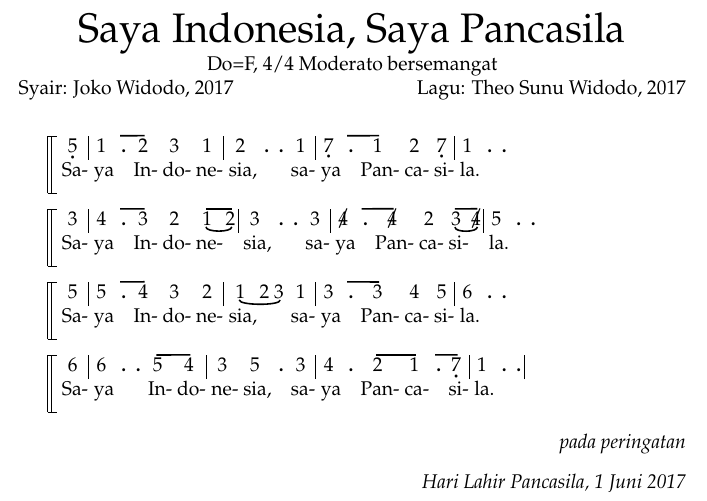
\includegraphics[scale=0.6]{saya-indonesia.png}
	\end{center}
\end{frame}

\begin{frame}{Doa Adven (Didoakan bergantian)}
\begin{enumerate}
\item [A] Langit dan bumi akan lenyap, tetapi sabdaMu, ya Tuhan,
akan tinggal tetap. Akan terpenuhilah janjimu; bahwa
Engkau akan datang lagi, mengadili orang yang hidup
maupun yang mati, dan mengganjar setiap orang, menurut
perbuatannya.
\item [B] Ya Tuhan, resapilah hati kami, dengan rasa takut yang
suci akan Dikau, dan akan keputusan hukummu, tetapi
juga dengan kerinduan yang hangat, akan kedatanganMu
yang menyelamatkan.
\end{enumerate}
\end{frame}

\begin{frame}{Doa Adven (Didoakan bergantian)}
	\begin{enumerate}
		\item [A] Dengan penuh kepercayaan akan belaskasihanMu, kami
		berharap, pada hari itu akan bangkit dengan penuh
		bahagia, dan berkata dengan gembira: lihatlah, penebusan
		kita sudah dekat.
		\item [B] Tuhan, janganlah biarkan kami tenggelam, di dalam hal-
		hal duniawi. Berilah kami selalu siap sedia, menantikan
		kedatanganMu, dengan lampu bernyala di tangan kami.
\end{enumerate}
\end{frame}

\begin{frame}{Doa Adven (Didoakan bergantian)}
	\begin{enumerate}
		\item [A] Bangunkanlah kami, sebab sudah tibalah saatnya, untuk
		bangun dari tidur, menanggalkan perbuatan-perbuatan
		kegelapan, dan mengenakan senjata terang.
		\item [B] Dengan doa penuh kepercayaan, dengan rasa takut yang
		suci, serta keyakinan sebagai anak kami rindu, akan
		menjumpai Dikau dengan penuh kegembiraan, apabila
		Engkau datang di atas awan-awan langit, untuk mengadili
		orang yang hidup, maupun yang mati. Amin
	\end{enumerate}
\end{frame}

\begin{frame}{Doa Penutup}
Ya Bapa yang Agung, Engkau telah memberikan kami
terang Kasih, khususnya Engkau telah menyadarkan kami
tentang nilai sila kedua dan kelima Pancasila, mengenai
nilai kemanusiaan dan keadilan. Kami sebagai warga
Indonesia, melalui pertemuan ini, semakin Engkau
sadarkan untuk senantiasa senantiasa menjunjung
martabat manusia dan rasa keadilan bagi semua orang,
tanpa pandang bulu, khususnya dalam hidup
bermasyarakat kami. Semoga kami semakin mampu
membangun semangat Pancasila di tengah-tengah hidup
bermasyarakat kami. Engkau yang hidup dan meraja, kini
dan sepanjang masa

Amin
\end{frame}

\end{document}